\subsection{Opsamling og behandling af EMG-signaler} \label{sec:EMG_imp}
For at opfylde de krav, der er opstillet i \autoref{sec:EMG_krav}, anvendes Muscle Sensor V3 fra Advancer Technologies, der fremover refereres til som 'EMG-forstærker'. 
Denne komponent måler en differens mellem de elektriske potentialer, der måles gennem elektroderne. 
EMG-forstærkeren består af en differensforstærker, et passivt højpasfilter, en helbølgeensretter, et aktivt lavpasfilter og en justerbar forstærker \citep{advancertech2013}. 

En illustration af, hvordan EMG-forstærkeren behandler et inputsignal fremgår af \autoref{fig:sinussignal}.
\begin{figure}[H]
\centering
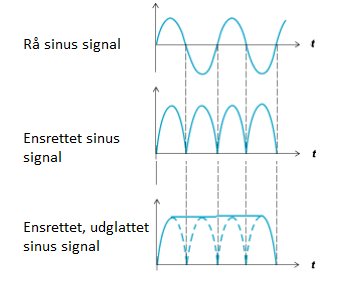
\includegraphics[width=0.6\textwidth]{figures/sinussignal.png}
\caption{Tre sinussignaler. Henholdsvis et råt, et ensrettet og et ensrettet samt udglattet sinussignal \citep{advancertech2013}.}
\label{fig:sinussignal}
\end{figure}

\noindent
På \autoref{fig:sinussignal} kan sinussignalet tolkes som et muskelsignal. 
Signalet passerer et passivt højpasfilter, der dæmper DC-støjen og dermed offsettet i signalet, hvilket medfører, at signalet centreres omkring 0. Dette fremgår af den øverste graf på \autoref{fig:sinussignal}. 
Centreringen er nødvendig for hensigtsmæssigt at ensrette signalet, da det ensrettes omkring tidsaksen. 
Denne ensretning er en helbølgeensretning, hvilket ses af den midterste graf på \autoref{fig:sinussignal}. 
Helbølgeensretning sker ved at invertere signalets negative værdier, således signalet kun har udslag i positiv retning. %Dette betyder at der ikke sker ændringer i det oprindelige signals energi. 
Herefter envelopefiltreres signalet, hvilket ses som det udglattede signal på nederste graf i \autoref{fig:sinussignal}. 

Envelopefiltret har til formål at stabilisere signalet, hvilket er implementeret i EMG-forstærkeren ved et lavpasfilter. 
Filtreret er beregnet til at have en knækfrekvens ($f_c$) på $1,94~Hz$ ud fra \autoref{eq:lavcutfre}. 
Denne  beregnes ud fra filtrerets modstande ($R$) og kondensatorer ($C$). 
Disse værdier er fundet i databladet for EMG-forstærkeren, hvor $C$ er aflæst til $1 \cdot 10^{-6}~F$ og $R$ til $80,6 \cdot 10^3~\Omega$ \citep{advancertech2013}. 

\begin{equation}\label{eq:lavcutfre}
f_c = \frac{1}{2 \pi C R} = \frac{1}{2 \pi \cdot 1 \cdot 10^{-6}~F \cdot 80,6 \cdot 10^3~\Omega} = 1,94~Hz
\end{equation}

\noindent
For at sikre, at EMG-forstærkerens forstærkning, ensretning og udglatning fungerer, kræver EMG-forstærkeren en spændingsforsyning på minimum $\pm 3~V$ og maksimalt $\pm 30~V$. Herudover er der mulighed for at justere modstanden fra $0,1~\Omega$ til $100~k\Omega$, hvilket giver et justerbart gain fra 0,002 til 20.700 gange, såfremt den forsynes med en spænding på $\pm 30~V$ \citep{advancertech2013}. 